\chapter{Síntesis total: estrategia y rutas clásicas}\label{ch:b3:total-synthesis}

El fármaco anticanceroso paclitaxel se aisló por primera vez de la corteza del tejo del
Pacífico, un árbol de crecimiento lento; descortezarlo mataba el árbol, y el suministro quedaba
muy por debajo de lo que necesitaban los pacientes. Los químicos respondieron de dos maneras: con \omterm{def:b3:total-synthesis:total}{síntesis
totales}, que demostraron que la molécula podía construirse a partir de materiales de partida
sencillos pero eran demasiado largas para la producción, y con una \omterm{def:b3:total-synthesis:total}{semisíntesis} a partir de un
compuesto emparentado extraído de las acículas de un tejo común, que es renovable.
Este capítulo trata de cómo se juzgan y se diseñan esas rutas: cómo se multiplican los
rendimientos, por qué compensa la convergencia, cuánto cuestan los grupos protectores, qué enlaces
formar primero, y tres síntesis emblemáticas leídas con esas herramientas.

\begin{recall}
El volumen del segundo año trató el análisis retrosintético (molécula objetivo,
desconexión, sintón, equivalente sintético, interconversión de grupos
funcionales), los grupos protectores ortogonales, la reacción aldólica, la
anelación de Robinson, la reacción de Wittig y la química de los iones iminio; el volumen del
primer año, los grupos protectores y los rendimientos. Los \cref{ch:b3:asymmetric-synthesis},
\cref{ch:b3:pericyclic} y \cref{ch:b3:homogeneous-catalysis} aportaron las
etapas clave modernas.
\end{recall}

\begin{omfigure}
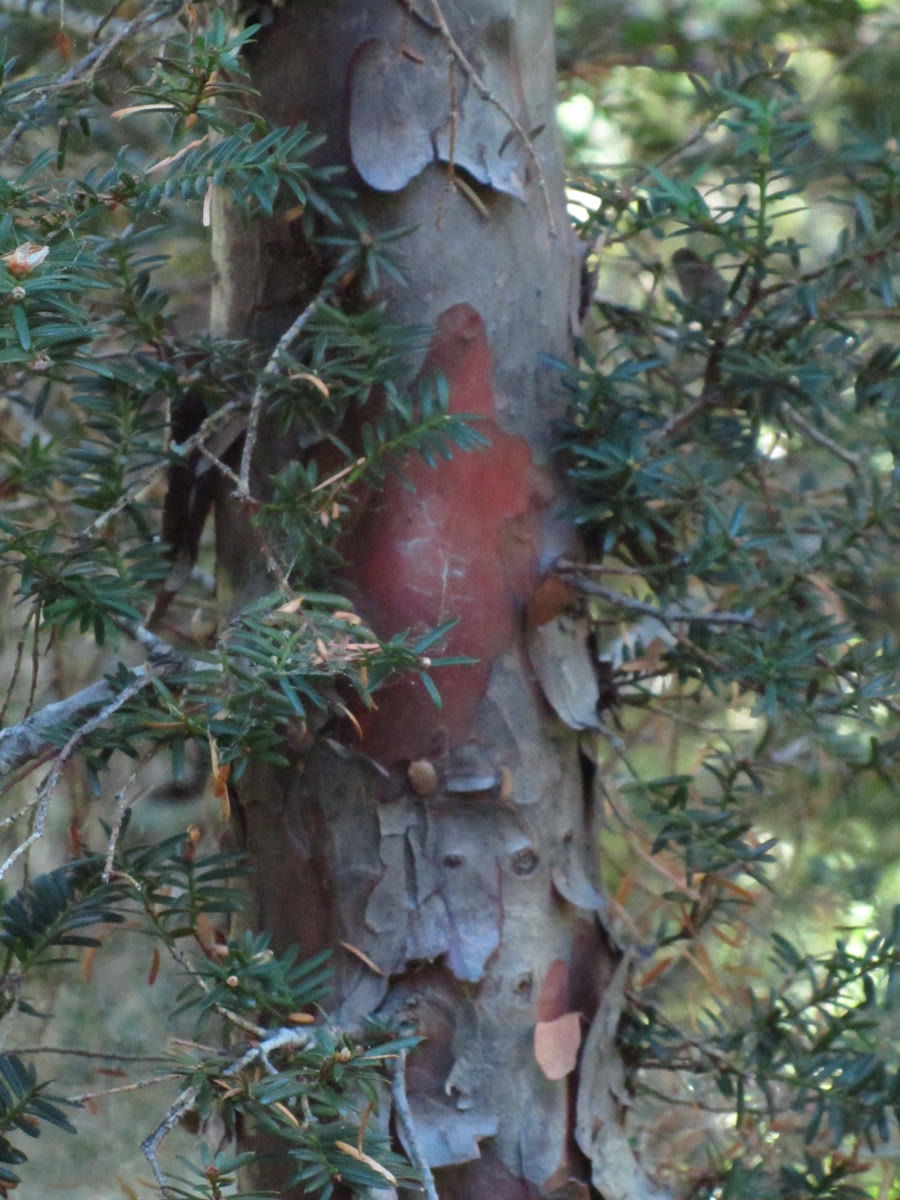
\includegraphics[width=0.32\linewidth]{images/book4/pacific-yew.jpg}

{\small Corteza y acículas de un tejo del Pacífico, la primera fuente de paclitaxel.
Fotografía: JOE BLOWE, CC BY-SA 2.0.}
\end{omfigure}

\section{Medir una síntesis}

\begin{definition}[Síntesis total]\label{def:b3:total-synthesis:total}
Una \emph{síntesis total}\index{sintesis total@síntesis total} prepara una molécula compleja, a menudo
un producto natural, a partir de compuestos comerciales sencillos. Una \emph{síntesis
formal}\index{sintesis formal@síntesis formal} prepara un intermedio de una síntesis total
anterior, con lo que completa la ruta sobre el papel. Una \emph{semisíntesis}\index{semisintesis@semisíntesis}
parte de un compuesto natural ya próximo a la molécula objetivo.
\end{definition}

\begin{definition}[Arquitectura de una ruta]\label{def:b3:total-synthesis:architecture}
En una \emph{síntesis lineal}\index{sintesis lineal@síntesis lineal}, cada etapa actúa sobre el
producto de la anterior; en una \emph{síntesis convergente}\index{sintesis convergente@síntesis convergente},
se preparan fragmentos separados en paralelo que se unen al final. La
\emph{secuencia lineal más larga}\index{secuencia lineal mas larga@secuencia lineal más larga} (LLS) es el
mayor número de etapas desde cualquier material de partida hasta la molécula objetivo. El
\emph{rendimiento global}\index{rendimiento global} es la cantidad de producto final obtenida
dividida por la cantidad del material de partida limitante.
\end{definition}

\begin{proposition}[Rendimiento global]\label{prop:b3:total-synthesis:overall-yield}
Para una secuencia de etapas de rendimientos $y_1, \dots, y_n$, el \omterm{def:b3:total-synthesis:architecture}{rendimiento global} es $Y = \prod_i y_i$.
\end{proposition}

\begin{proof}
Cada etapa convierte la cantidad que recibe en $y_i$ veces esa cantidad de producto; la
cantidad que llega a la molécula objetivo es la cantidad inicial multiplicada sucesivamente por cada
factor.
\end{proof}

\begin{proposition}[Convergencia]\label{prop:b3:total-synthesis:convergent}
Una ruta de $n = 2m + 1$ etapas de igual rendimiento $y$, construida como dos ramas de $m$ etapas unidas por
una etapa de acoplamiento, tiene el \omterm{def:b3:total-synthesis:architecture}{rendimiento global} $y^{m+1}$ a lo largo de su \omterm{def:b3:total-synthesis:architecture}{secuencia lineal más larga},
frente a $y^{2m+1}$ para la ruta lineal con las mismas etapas.
\end{proposition}

\begin{proof}
Cada rama se prepara por separado, con tanto material de partida como haga falta: el
material de cada rama pasa por $m$ etapas y después por el acoplamiento, $m + 1$
factores $y$. En la ruta lineal, el material pasa por las $2m + 1$. Para $m = 10$
e $y = 0.90$: 31\,\% frente a 11\,\%.
\end{proof}

\begin{omfigure}
\begin{tikzpicture}
\begin{axis}[width=0.7\linewidth, height=5.8cm, xmin=0, xmax=30, ymin=0, ymax=1.02,
  axis lines=left, xlabel={número de etapas $n$}, ylabel={rendimiento global},
  tick label style={font=\scriptsize}, label style={font=\small},
  legend style={font=\scriptsize, draw=none, at={(1.03,0.5)}, anchor=west}, legend cell align=left]
\addplot[color=omDef, thick] table[x=n, y=y95] {figdata/out/bachelor-3-overall-yield.dat};
\addlegendentry{95\,\% por etapa}
\addplot[color=omMeth, thick] table[x=n, y=y90] {figdata/out/bachelor-3-overall-yield.dat};
\addlegendentry{90\,\%}
\addplot[color=omThm, thick] table[x=n, y=y80] {figdata/out/bachelor-3-overall-yield.dat};
\addlegendentry{80\,\%}
\addplot[color=omMeth, thick, dashed, mark=*, mark size=1pt] table[x=n, y=y90] {figdata/out/bachelor-3-overall-yield-b.dat};
\addlegendentry{90\,\%, convergente}
\end{axis}
\end{tikzpicture}

{\small \omterm{def:b3:total-synthesis:architecture}{Rendimiento global} en función del número de etapas para tres rendimientos por etapa
(trazo continuo: rutas lineales), y para rutas convergentes al 90\,\% por etapa (dos ramas
iguales unidas en una última etapa; trazo discontinuo). Veinte etapas al 90\,\% dejan un 12\,\%; las
mismas etapas dispuestas de forma convergente dejan unas tres veces más.}
\end{omfigure}

\begin{omfigure}
\begin{tikzpicture}[font=\scriptsize, >=Stealth, node distance=0.9cm,
  st/.style={circle, draw, fill=omDef!15, minimum size=4mm, inner sep=0pt}]
  \foreach \i in {0,...,6} { \node[st] (l\i) at (\i*0.9,1.6) {}; }
  \foreach \i in {0,...,5} { \pgfmathtruncatemacro\j{\i+1} \draw[->] (l\i) -- (l\j); }
  \node[anchor=west] at (6.0,1.6) {lineal: 6 etapas, LLS 6};
  \foreach \i in {0,...,2} { \node[st] (a\i) at (\i*0.9,0.6) {}; \node[st] (b\i) at (\i*0.9,-0.6) {}; }
  \draw[->] (a0) -- (a1); \draw[->] (a1) -- (a2); \draw[->] (b0) -- (b1); \draw[->] (b1) -- (b2);
  \node[st, fill=omThm!25] (t) at (3.0,0) {};
  \draw[->] (a2) -- (t); \draw[->] (b2) -- (t);
  \node[anchor=west] at (3.4,0) {convergente: 5 etapas, LLS 3};
\end{tikzpicture}

{\small Árboles de ruta: cada círculo es un compuesto, y cada flecha, una etapa. Una ruta lineal
hace pasar todo su material por todas las etapas; una convergente prepara dos fragmentos
en paralelo y los acopla, de modo que su \omterm{def:b3:total-synthesis:architecture}{secuencia lineal más larga} es más corta.}
\end{omfigure}

\begin{definition}[Economías e idealidad]\label{def:b3:total-synthesis:economy}
La \emph{economía de etapas}\index{economia de etapas@economía de etapas} es el objetivo de alcanzar una molécula objetivo en el menor
número posible de etapas; la \emph{economía de grupos protectores}\index{economia de grupos protectores@economía de grupos protectores},
el de usar el menor número posible de etapas de protección y desprotección. La
\emph{idealidad}\index{idealidad} de una ruta es la fracción de sus etapas que
construyen el esqueleto o realizan un cambio necesario del nivel de oxidación:
$(\text{etapas de construcción} + \text{etapas redox estratégicas})/(\text{etapas totales})$.
\end{definition}

\begin{proposition}[Idealidad de una ruta]\label{prop:b3:total-synthesis:ideality}
Una ruta en un solo recipiente que solo forma enlaces del esqueleto tiene una \omterm{def:b3:total-synthesis:economy}{idealidad} del 100\,\%; cada etapa de protección,
de desprotección, de interconversión de grupos funcionales o redox no estratégica
la reduce.
\end{proposition}

\begin{proof}
Se deduce directamente de la definición: esas etapas se suman al denominador sin sumarse
al numerador.
\end{proof}

\section{Los grupos protectores y su economía}

Cada grupo protector cuesta al menos dos etapas, los reactivos para introducirlo y
eliminarlo, y el material perdido en ambas. Una ruta de ocho etapas al 90\,\% conserva
el 43\,\% de su material; añadir dos protecciones y dos desprotecciones al 95\,\% cada una
lo reduce al 35\,\%. Los grupos protectores se eligen ortogonales, de modo que cada uno pueda
eliminarse sin tocar los demás; mejor aún, el orden de las etapas se
dispone de modo que el grupo reactivo no esté presente, o no se haya revelado todavía, cuando
interferiría: las síntesis sin grupos protectores son un objetivo, no una curiosidad.

\begin{method}[Leer una síntesis total]\label{met:b3:total-synthesis:analyse}
\begin{enumerate}
  \item Identificar los anillos, los estereocentros y los grupos sensibles de la molécula objetivo.
  \item Encontrar las desconexiones clave y las reacciones que las realizan en sentido
        directo (\omterm{def:b3:total-synthesis:strategic-bond}{enlaces estratégicos}).
  \item Contar las etapas y encontrar la \omterm{def:b3:total-synthesis:architecture}{secuencia lineal más larga}; anotar la convergencia.
  \item Anotar cómo se fija cada estereocentro (control por el sustrato, auxiliar, catalizador,
        \omterm{def:b3:asymmetric-synthesis:chiral-pool}{acervo quiral}).
  \item Enumerar los grupos protectores y las demás etapas no ideales; calcular el \omterm{def:b3:total-synthesis:architecture}{rendimiento
        global} y la \omterm{def:b3:total-synthesis:economy}{idealidad}.
\end{enumerate}
\end{method}

\begin{method}[Contar las etapas]\label{met:b3:total-synthesis:count}
\begin{enumerate}
  \item Una etapa es una operación que termina en un producto aislado (o al menos sometido a tratamiento);
        una secuencia en un solo recipiente sin aislamiento cuenta como una etapa.
  \item Contar todas las etapas para el total; para la LLS, seguir el camino más largo desde un
        compuesto comercial hasta la molécula objetivo.
  \item Multiplicar los rendimientos a lo largo de la LLS para obtener el \omterm{def:b3:total-synthesis:architecture}{rendimiento global}.
\end{enumerate}
\end{method}

\section{Enlaces estratégicos y etapas clave de formación de anillos}

\begin{definition}[Enlace estratégico]\label{def:b3:total-synthesis:strategic-bond}
Un \emph{enlace estratégico} de una molécula objetivo\index{enlace estrategico@enlace estratégico} es un enlace cuya
desconexión simplifica más la molécula, normalmente al dividir un sistema de anillos
o eliminar varios estereocentros a la vez, y que una reacción fiable puede
formar.
\end{definition}

Las reacciones de formación de anillos que forman dos enlaces o varios estereocentros a la vez
son los caballos de batalla: la reacción de Diels--Alder (dos enlaces C--C, hasta cuatro
estereocentros, de forma estereoespecífica, \cref{ch:b3:pericyclic}), la anelación de
Robinson (un anillo de seis miembros sobre una cetona), la \omterm{def:b3:homogeneous-catalysis:metathesis}{metátesis por cierre de anillo}
(\cref{ch:b3:homogeneous-catalysis}) para los anillos medianos y grandes, y las cascadas.

\begin{definition}[Reacción en cascada]\label{def:b3:total-synthesis:cascade}
Una \emph{reacción en cascada}\index{reaccion en cascada@reacción en cascada} es una secuencia de
transformaciones en la que cada etapa crea la funcionalidad necesaria para la siguiente,
sin aislar intermedios ni añadir reactivos.
\end{definition}

\begin{definition}[Síntesis biomimética]\label{def:b3:total-synthesis:biomimetic}
Una \emph{síntesis biomimética}\index{sintesis biomimetica@síntesis biomimética} imita la ruta
por la que se cree que el organismo fabrica un producto natural.
\end{definition}

La ciclación del óxido de escualeno a lanosterol en las células, cuatro anillos y siete
estereocentros en una sola cascada enzimática, inspiró las ciclaciones de polienos de
William Johnson, en las que un catión iniciado en un extremo de un polieno cuidadosamente
diseñado cierra un anillo tras otro a través de estados de transición de tipo silla, fijando
las fusiones de anillo \textit{trans} de los esteroides.

\section{Rutas emblemáticas}

\begin{definition}[Reacción de Mannich]\label{def:b3:total-synthesis:mannich}
La \emph{reacción de Mannich}\index{reaccion de Mannich@reacción de Mannich} es la adición de un enol
o de un enolato a un ion iminio, formado in situ a partir de un aldehído y de una amina primaria o
secundaria, que da un compuesto $\beta$-aminocarbonílico.
\end{definition}

En 1917, Robert Robinson preparó la tropinona, el núcleo bicíclico de la atropina y de la
cocaína, en un solo recipiente a partir de tres componentes sencillos en agua, imaginando que la
planta podría construirla del mismo modo:
$\ce{C4H6O2 + CH3NH2 + C5H6O5 -> C8H13NO + 2CO2 + 2H2O}$ (el succinaldehído, la metilamina y el
ácido acetonadicarboxílico dan la tropinona).

\begin{omfigure}
\begin{tikzpicture}[font=\small, >=Stealth]
  \node[align=center] at (-0.5,0) {$\ce{OHC-CH2CH2-CHO}$\\ $+\ \ce{CH3NH2}$\\ $+\ \ce{HO2C-CH2-CO-CH2-CO2H}$};
  \draw[->, thick] (3.0,0) -- (4.7,0) node[midway, above, font=\scriptsize] {agua tamponada} node[midway, below, font=\scriptsize] {$-\ce{2CO2}$, $-\ce{2H2O}$};
  \begin{scope}[xshift=6.1cm, yshift=-0.2cm]
    \coordinate (c1) at (-1,0.3); \coordinate (c2) at (-0.8,-0.5); \coordinate (c3) at (0,-0.9);
    \coordinate (c4) at (0.8,-0.5); \coordinate (c5) at (1,0.3); \coordinate (c6) at (0.45,1.15);
    \coordinate (c7) at (-0.45,1.15); \coordinate (n) at (0,0.45);
    \draw[thick] (c1) -- (c2) -- (c3) -- (c4) -- (c5) -- (c6);
    \draw[thick] (c7) -- (c1);
    \draw[thick] (c6) -- (0.12,1.15); \draw[thick] (-0.12,1.15) -- (c7);
    \draw[thick] (c1) -- (n) -- (c5);
    \draw[thick] (n) -- (0,1.6) node[above, inner sep=1pt] {$\ce{CH3}$};
    \draw[thick, double, double distance=1.5pt] (c3) -- (0,-1.55) node[below, inner sep=1pt] {O};
    \node[fill=white, inner sep=0.5pt] at (n) {N};
    \node[font=\scriptsize, anchor=west] at (1.2,0.3) {tropinona};
  \end{scope}
\end{tikzpicture}

{\small Síntesis de la tropinona de Robinson. Dos \omterm{def:b3:total-synthesis:mannich}{reacciones de Mannich}, la primera
intermolecular y la segunda de cierre de anillo, unen los tres componentes;
los dos grupos ácido carboxílico que hacían enolizables los grupos $\ce{CH2}$ centrales se
van después como dióxido de carbono. En el producto bicíclico, el puente N-metilo atraviesa el
anillo de siete miembros.}
\end{omfigure}

\begin{proposition}[La tropinona en un solo recipiente]\label{prop:b3:total-synthesis:tropinone}
La síntesis de la tropinona en un solo recipiente consiste en dos \omterm{def:b3:total-synthesis:mannich}{reacciones de Mannich} seguidas de dos
descarboxilaciones.
\end{proposition}

\begin{proof}[Argumento]
La metilamina y uno de los grupos aldehído del succinaldehído dan un ion iminio; un
enol del ácido acetonadicarboxílico se adiciona a él (primera \omterm{def:b3:total-synthesis:mannich}{reacción de Mannich}). La amina
secundaria formada se condensa con el segundo grupo aldehído en un ion iminio
cíclico, al que ataca el enol del otro lado de la cetona (segunda \omterm{def:b3:total-synthesis:mannich}{reacción de Mannich}),
lo que cierra el biciclo. Los dos grupos $\beta$-cetoácido pierden después $\ce{CO2}$, como hacen los $\beta$-cetoácidos
al calentarlos suavemente.
\end{proof}

La síntesis de la prostaglandina $\mathrm F_{2\alpha}$ de Elias Corey (1969) hizo explícito el análisis retrosintético.
Una biciclo[2.2.1]heptenona construida mediante una reacción de Diels--Alder lleva
la configuración relativa de los sustituyentes del ciclopentano; una
\omterm{def:b3:radicals-carbenes:baeyer}{oxidación de Baeyer--Villiger} (\cref{ch:b3:radicals-carbenes}) y una
yodolactonización la convierten en la lactona de Corey, a la que se unen las dos cadenas laterales
mediante olefinaciones. La lactona ha servido desde entonces para muchos fármacos
prostaglandínicos.

\begin{omfigure}
\begin{tikzpicture}[font=\small,
  box/.style={draw, rounded corners, align=center, fill=omDef!8, inner sep=4pt}]
  \node[box] (t) at (-0.6,0) {prostaglandina\\ $\mathrm F_{2\alpha}$};
  \node[box] (l) at (4.4,0) {lactona de Corey\\ (cuatro\\ estereocentros)};
  \node[box] (b) at (9.8,0) {biciclo[2.2.1]-\\ heptenona};
  \node[box] (d) at (9.8,-2.4) {ciclopentadieno\\ sustituido $+$\\ equivalente de ceteno};
  \draw[omretro] (t) -- (l) node[midway, above=3pt, font=\scriptsize] {olefinaciones};
  \draw[omretro] (l) -- (b) node[midway, above=3pt, font=\scriptsize, align=center] {yodolactonización,\\ Baeyer--Villiger};
  \draw[omretro] (b) -- (d) node[midway, right, font=\scriptsize] {Diels--Alder};
\end{tikzpicture}

{\small Retrosíntesis de la prostaglandina $\mathrm F_{2\alpha}$ de Corey, a grandes rasgos (flechas dobles: ``se
obtiene a partir de''). Las dos cadenas laterales se desconectan primero; el ciclopentano con
sus cuatro estereocentros procede de una lactona; la lactona, de una cetona bicíclica,
y la cetona, de una reacción de Diels--Alder que fija su configuración
relativa.}
\end{omfigure}

El oseltamivir, el fármaco contra la gripe, se fabrica industrialmente a partir del ácido shikímico, un
compuesto del \omterm{def:b3:asymmetric-synthesis:chiral-pool}{acervo quiral} extraído del anís estrellado y producido después por
fermentación: su anillo de seis miembros y sus estereocentros ya están en su sitio.
La ruta convierte el diol del anillo en un epóxido, lo abre con azida, cierra una
aziridina y la abre de nuevo con azida, lo que sitúa los dos átomos de nitrógeno
en \textit{trans}; la acetilación y la reducción terminan el trabajo. Como la azida de sodio y
las azidas orgánicas son tóxicas y potencialmente explosivas a gran escala, más tarde se desarrollaron
rutas sin azida.

\begin{omfigure}
\begin{tikzpicture}[font=\scriptsize, >=Stealth,
  box/.style={draw, rounded corners, align=center, fill=omMeth!8, inner sep=3pt}]
  \node[box] (a) at (0,0) {ácido ($-$)-shikímico\\ (acervo quiral)};
  \node[box] (b) at (3.1,0) {éster, cetal,\\ mesilato};
  \node[box] (c) at (6.0,0) {epóxido};
  \node[box] (d) at (8.6,0) {azidoalcohol};
  \node[box] (e) at (8.6,-1.5) {aziridina};
  \node[box] (f) at (5.4,-1.5) {precursor de la\\ \textit{trans}-diamina (azida)};
  \node[box] (g) at (1.0,-1.5) {fosfato de\\ oseltamivir};
  \draw[->] (a) -- (b); \draw[->] (b) -- (c); \draw[->] (c) -- (d) node[midway, above] {$\ce{N3-}$};
  \draw[->] (d) -- (e); \draw[->] (e) -- (f) node[midway, above] {$\ce{N3-}$};
  \draw[->] (f) -- (g) node[midway, below, align=center] {acetilación,\\ reducción};
\end{tikzpicture}

{\small El oseltamivir a partir del ácido shikímico, solo las etapas clave: se conservan el anillo natural y sus
estereocentros, y se introducen dos átomos de nitrógeno en \textit{trans} entre sí
mediante aperturas sucesivas de un epóxido y de una aziridina con azida.}
\end{omfigure}

\section{Del descubrimiento al proceso}

Una ruta que proporciona miligramos para los ensayos biológicos rara vez es la que se usa
para fabricar toneladas. Los químicos de procesos exploran las rutas según su coste, su seguridad y su robustez:
sustituyen la cromatografía por la cristalización, reemplazan los reactivos peligrosos
y las temperaturas criogénicas, acortan la secuencia, comprueban la seguridad
térmica de cada etapa por calorimetría y fijan especificaciones para las impurezas.
Estas elecciones se corresponden con las medidas del \cref{ch:b3:green-industrial}.

\begin{inthelab}[De un gramo a un kilogramo]
Una etapa realizada con un gramo en un matraz de fondo redondo se repite con diez gramos en un
reactor encamisado con agitador mecánico y una sonda de temperatura en el
líquido, añadiendo el reactivo más reactivo a una velocidad controlada mientras se vigila la
temperatura interna: el calor liberado crece con el volumen, pero la superficie que lo
evacua solo crece con el cuadrado del tamaño. Solo cuando el flujo de calor y el tratamiento
(separaciones de fases, filtraciones, secado) se comportan bien se realiza la etapa a escala de un kilogramo.
\end{inthelab}

\begin{safety}{\ghs[0.62cm]{GHS06}\ghs[0.62cm]{GHS08}\ghs[0.62cm]{GHS09}}
% ledger: ghs4:NaN3
Azida de sodio: mortal en caso de ingestión, muy tóxica para los organismos acuáticos; con los ácidos
libera ácido hidrazoico, un gas tóxico y explosivo, y con los metales pesados
(el cobre y el plomo de los desagües) forma azidas explosivas. Los residuos se destruyen
químicamente; nunca se vierten.
\end{safety}

\begin{history}[Robinson, Woodward, Corey]
Robert Robinson recibió el Premio Nobel de Química de 1947 por sus trabajos sobre los
alcaloides y otros productos vegetales; su síntesis de la tropinona de 1917 se sigue
citando por su economía. Las síntesis de Robert Woodward de la quinina, el colesterol, la
clorofila y, con Albert Eschenmoser, la vitamina $\mathrm B_{12}$ hicieron de la \omterm{def:b3:total-synthesis:total}{síntesis total} un arte
(premio de 1965). Elias Corey formalizó el análisis retrosintético y recibió el
premio de 1990 por la teoría y la metodología de la síntesis orgánica.
\end{history}

\section{Ejercicios}

\begin{exercise}[$\star$]\label{exo:b3:total-synthesis:1}
Calcúlese el \omterm{def:b3:total-synthesis:architecture}{rendimiento global} de rutas lineales de 10 y de 20 etapas al 90\,\% y al 80\,\% por
etapa.
\end{exercise}

\begin{exercise}[$\star$]\label{exo:b3:total-synthesis:2}
Una ruta prepara el fragmento A en cinco etapas y el fragmento B en tres, los acopla y
necesita cuatro etapas más hasta la molécula objetivo. Dense el número total de etapas y la
\omterm{def:b3:total-synthesis:architecture}{secuencia lineal más larga}.
\end{exercise}

\begin{exercise}[$\star$]\label{exo:b3:total-synthesis:3}
Dese el producto de la \omterm{def:b3:total-synthesis:mannich}{reacción de Mannich} de la acetona, el formaldehído y la
dimetilamina.
\end{exercise}

\begin{exercise}[$\star$]\label{exo:b3:total-synthesis:4}
Dese una desconexión de Diels--Alder del 4-acetilciclohexeno, y la reacción
directa.
\end{exercise}

\begin{exercise}[$\star\star$]\label{exo:b3:total-synthesis:5}
Una ruta lineal de 21 etapas transcurre al 90\,\% por etapa. Calcúlense su \omterm{def:b3:total-synthesis:architecture}{rendimiento global} y el
de una versión convergente con dos ramas de 10 etapas y un acoplamiento.
\end{exercise}

\begin{exercise}[$\star\star$]\label{exo:b3:total-synthesis:6}
La ruta A tiene 12 etapas, de las cuales 7 forman enlaces del esqueleto y 1 es una reducción
estratégica; la ruta B tiene 9 etapas, 7 de ellas de esqueleto. Calcúlense sus \omterm{def:b3:total-synthesis:economy}{idealidades}.
\end{exercise}

\begin{exercise}[$\star\star$]\label{exo:b3:total-synthesis:7}
Una ruta de ocho etapas al 90\,\% por etapa necesita dos grupos protectores, cada uno introducido y
eliminado al 95\,\%. Calcúlese el \omterm{def:b3:total-synthesis:architecture}{rendimiento global} con ellos y sin ellos.
\end{exercise}

\begin{exercise}[$\star\star$]\label{exo:b3:total-synthesis:8}
Un triol tiene un grupo hidroxi primario, uno secundario y uno terciario. Propónganse
grupos protectores que permitan revelar cada uno por turno, y sus condiciones de
eliminación.
\end{exercise}

\begin{exercise}[$\star\star$]\label{exo:b3:total-synthesis:9}
¿Por qué el paclitaxel se produjo por \omterm{def:b3:total-synthesis:total}{semisíntesis} y no mediante ninguna de sus \omterm{def:b3:total-synthesis:total}{síntesis
totales}?
\end{exercise}

\begin{exercise}[$\star\star\star$]\label{exo:b3:total-synthesis:10}
La 2-metilciclohexano-1,3-diona reacciona con la metil vinil cetona en una anelación de
Robinson. Identifíquense las etapas de Michael y aldólica y dese la enona bicíclica
formada (la cetona de Wieland--Miescher).
\end{exercise}

\begin{exercise}[$\star\star\star$]\label{exo:b3:total-synthesis:11}
Demuéstrese que la ruta convergente de la \cref{prop:b3:total-synthesis:convergent} conserva
$y^{-m}$ veces más material que la lineal, y evalúese este factor para $m = 5$ y
$m = 15$ al 90\,\%.
\end{exercise}

\begin{exercise}[$\star\star\star$]\label{exo:b3:total-synthesis:12}
En una ciclación de polienos, ¿por qué los estados de transición de tipo silla dan fusiones de anillo
\textit{trans}, y por qué importa la geometría (\textit{E} o \textit{Z}) de cada doble enlace?
\end{exercise}

\section{Problema: la tropinona en un solo recipiente}

\begin{problem}[{Problema de fin de semana --- la tropinona en un solo recipiente: los tres componentes
y la ecuación ajustada, las dos reacciones de Mannich, una comparación con una larga
ruta lineal, y la estereoquímica de la tropinona y de sus productos de reducción}]
\label{pb:b3:total-synthesis:1}
% ledger: aw:C, aw:H, aw:N, aw:O
Datos del problema: la síntesis en un solo recipiente, realizada en agua tamponada cerca de pH 5,
da tropinona con un rendimiento del 42\,\%; una ruta lineal más antigua necesita 14 etapas con un rendimiento medio del 75\,\%.

\medskip\noindent\textbf{Parte I --- Componentes y ecuación.}
\begin{enumerate}
  \item Dense las fórmulas del succinaldehído, la metilamina, el ácido acetonadicarboxílico
        y la tropinona.
  \item Escríbase la ecuación ajustada.
  \item Calcúlense las masas molares de los reactivos y de la tropinona.
  \item Calcúlese la economía atómica.
  \item ¿Por qué se usa ácido acetonadicarboxílico en lugar de acetona?
  \item ¿Por qué ayuda tamponar cerca de un pH neutro?
\end{enumerate}

\medskip\noindent\textbf{Parte II --- Mecanismo.}
\begin{enumerate}[resume]
  \item Escríbase la formación del primer ion iminio.
  \item Muéstrese la primera \omterm{def:b3:total-synthesis:mannich}{reacción de Mannich}.
  \item ¿Cómo se forma el segundo ion iminio?
  \item Muéstrese la segunda \omterm{def:b3:total-synthesis:mannich}{reacción de Mannich}, que cierra el anillo.
  \item ¿Por qué los dos grupos ácido carboxílico se van como $\ce{CO2}$?
  \item Cuéntense los enlaces C--C y C--N formados.
\end{enumerate}

\medskip\noindent\textbf{Parte III --- Un solo recipiente frente a catorce etapas.}
\begin{enumerate}[resume]
  \item Calcúlese el \omterm{def:b3:total-synthesis:architecture}{rendimiento global} de la ruta lineal.
  \item Calcúlese la razón entre el rendimiento en un solo recipiente y este.
  \item Calcúlese la \omterm{def:b3:total-synthesis:economy}{idealidad} de la ruta en un solo recipiente.
  \item ¿Qué otra cosa, además del rendimiento, favorece la ruta en un solo recipiente?
  \item ¿Por qué se dice que la síntesis en un solo recipiente es biomimética?
  \item Nómbrese otra clase de reacciones de este capítulo que forme varios enlaces a la vez.
\end{enumerate}

\medskip\noindent\textbf{Parte IV --- Estereoquímica.}
\begin{enumerate}[resume]
  \item ¿Es quiral la tropinona? Encuéntrese su \omterm{def:b3:point-groups:operation}{elemento de simetría}.
  \item ¿Por qué los dos carbonos cabeza de puente son, sin embargo, estereocentros?
  \item La reducción de la cetona da dos alcoholes, la tropina y la pseudotropina. ¿Qué
        relación hay entre ellos?
  \item ¿Son quirales la tropina y la pseudotropina?
  \item ¿Por qué un hidruro se aproxima al grupo carbonilo preferentemente por una cara?
  \item Enúnciese el resultado: la razón entre el rendimiento en un solo recipiente y el \omterm{def:b3:total-synthesis:architecture}{rendimiento
        global} de la ruta lineal.
\end{enumerate}
\end{problem}
